\documentclass[times,english,brazil,oneside, a4paper, fleqn]{ifes8}

\usepackage[utf8]{inputenc}
\usepackage{lastpage}           % Usado pelo exemplo de ficha catalográfica
\usepackage[alf, abnt-thesis-year=both]{abntex2cite}
\usepackage{microtype}          % para melhorias de justificação
\usepackage{morefloats}         % permite mais floats
\usepackage{listings}
\usepackage[table]{xcolor}
\usepackage{tikz}
\usetikzlibrary[topaths]
\usepackage{mathtools}
\usepackage[final]{pdfpages}
\usepackage{amsmath}
\usepackage{subcaption}
\usepackage{multirow}
\usepackage{boxhandler}
\usepackage{longtable}
\usepackage{placeins}
\setlength {\marginparwidth }{2cm}
\usepackage{todonotes}
%\usepackage[none]{hyphenat}%não separar a silaba
\setlength\mathindent{0pt}
\usepackage{setspace}
\usepackage{float}
\usepackage{url}
\usepackage{hyperref}
\usepackage[bottom]{footmisc}



\definecolor{mygreen}{rgb}{0,0.6,0}
\definecolor{mygray}{rgb}{0.5,0.5,0.5}
\definecolor{mymauve}{rgb}{0.58,0,0.82}


%%% The \raggedbottom declaration makes all pages the height of the text on that page.
%%% No extra vertical space is added.
\raggedbottom



%%% Definição da linguagem padrão do documento (pacote babel) para
%%% definir que certas porções do texto (como o resumo, por exemplo)
%%% estão em uma língua estrangeira, usar as macros
%%% \foreignlanguage{languageB}{Text in another language}
%%% ou
%%% \begin{otherlanguage}{languageB}
%%% ...
%%% \end{otherlanguage}
\selectlanguage{brazil}

\setlength{\abovecaptionskip}{5pt} % espaçamento antes da legenda de tabelas/figuras



%%% Define que todos os códigos fontes construídos com o ambiente
%%% `lstlisting' terão uma borda simples.
\lstset{ %
  backgroundcolor=\color{white},   % choose the background color
  basicstyle=\footnotesize,        % size of fonts used for the code
  breaklines=true,                 % automatic line breaking only at whitespace
  captionpos=b,                    % sets the caption-position to bottom
  commentstyle=\color{mygreen},    % comment style
  escapeinside={\%*}{*)},          % if you want to add LaTeX within your code
  keywordstyle=\color{blue},       % keyword style
  stringstyle=\color{mymauve}, 
  numbers=left,
  stepnumber=1,    
  firstnumber=1,
  numberfirstline=true% string literal style,
   frame=top,frame=bottom, frame=single,
   captionpos=t,
   literate=
  {á}{{\'a}}1 {é}{{\'e}}1 {í}{{\'i}}1 {ó}{{\'o}}1 {ú}{{\'u}}1
  {Á}{{\'A}}1 {É}{{\'E}}1 {Í}{{\'I}}1 {Ó}{{\'O}}1 {Ú}{{\'U}}1
  {à}{{\`a}}1 {è}{{\`e}}1 {ì}{{\`i}}1 {ò}{{\`o}}1 {ù}{{\`u}}1
  {À}{{\`A}}1 {È}{{\'E}}1 {Ì}{{\`I}}1 {Ò}{{\`O}}1 {Ù}{{\`U}}1
  {ä}{{\"a}}1 {ë}{{\"e}}1 {ï}{{\"i}}1 {ö}{{\"o}}1 {ü}{{\"u}}1
  {Ä}{{\"A}}1 {Ë}{{\"E}}1 {Ï}{{\"I}}1 {Ö}{{\"O}}1 {Ü}{{\"U}}1
  {â}{{\^a}}1 {ê}{{\^e}}1 {î}{{\^i}}1 {ô}{{\^o}}1 {û}{{\^u}}1
  {Â}{{\^A}}1 {Ê}{{\^E}}1 {Î}{{\^I}}1 {Ô}{{\^O}}1 {Û}{{\^U}}1
  {œ}{{\oe}}1 {Œ}{{\OE}}1 {æ}{{\ae}}1 {Æ}{{\AE}}1 {ß}{{\ss}}1
  {ű}{{\H{u}}}1 {Ű}{{\H{U}}}1 {ő}{{\H{o}}}1 {Ő}{{\H{O}}}1
  {ç}{{\c c}}1 {Ç}{{\c C}}1 {ø}{{\o}}1 {å}{{\r a}}1 {Å}{{\r A}}1
  {€}{{\EUR}}1 {£}{{\pounds}}1
}


\newcommand{\ifestex}{\textsf{Ifes$8$}}

\titulo{COMPARAÇÃO DE TÉCNICAS DE REDUÇÃO DE DIMENSIONALIDADE APLICADA NA DETECÇÃO DE ANOMALIAS EM
POÇOS DE PETRÓLEO}
\autor{Bruno Kobi Valadares de Amorim}
\local{Serra}
\data{2022}
\orientador[Orientadora:]{Profª.Dra. Kelly Assis de Souza Gazolli}
\coorientador[Orientador:]{Prof. Dr. Hilário Seibel Júnior}


\instituicao{%
  Instituto Federal do Espírito Santo
 }

\curso{PROGRAMA DE PÓS-GRADUAÇÃO EM COMPUTAÇÃO APLICADA – PPCOMP}
\tipotrabalho{Dissertação (Mestrado)}
\preambulo{Anteprojeto apresentado ao Programa de Pós-Graduação em Computação Aplicada – PPCOMP do Instituto Federal do Espírito Santo, como requisito para aprovação da Disciplina de Pesquisa em Computação Aplicada.} 


\begin{document}

\setsecnumformat{\csname the#1\endcsname\space}
\renewcommand{\afterchapternum}{\hspace{-4pt}}

%%% A macro \pretextual não precisa ser explicitamente chamada porque
%%% o abntex2 aciona essa macro no início do documento.
%%% \pretextual

\imprimircapa
\addtocounter{page}{-1}

\imprimirfolhaderosto*

% A ficha catalográfica será entregue pela Biblioteca
%\includepdf{pdf/FichaMarcelo.pdf}


% ------------------------- Folha de Aprovação ------------------------- 
% Entregue no dia da defesa 
%\includepdf{pdf/aprova_marcelo.pdf}


%%% ====================================================================
%%% Ambiente para a escrita da dedicatória.
%\begin{dedicatoria}
  %\vspace*{\fill}
 %\hspace{0.3\textwidth}
  %\begin{minipage}[t][4cm]{0.8\textwidth} 
   %\textit{Dedicatória }  \\
   %\textit{Dedicatória }  \\
   %\textit{Dedicatória} 
  %\end{minipage}
%\end{dedicatoria}


%%% ====================================================================
%%% Agradecimentos
%\begin{agradecimentos}
%Agradeço à toda minha família, amigos, professores, e pessoas que ajudaram na realização deste trabalho. Sou imensamente grato pela paciência e incentivo.
%\end{agradecimentos}


%%% ====================================================================
%%% Epígrafe
%\begin{epigrafe}
 % \vspace*{20cm}
  %\begin{otherlanguage}{english}
   % \begin{flushright}
    %%	\textit{epigrafe}
      %\end{SingleSpace}
    %\end{flushright}
  %\end{otherlanguage}
%\end{epigrafe}


%%% ====================================================================
%%% Ambiente para resumo em português
%\begin{resumo}[RESUMO]
\vspace*{-6mm}

Palavras-chave: 
\end{resumo}

%%% ====================================================================
%%% Ambiente para resumo em inglês.
%\begin{resumo}[ABSTRACT]
\begin{otherlanguage}{english}
\vspace*{-6mm}


Keywords: 

  \end{otherlanguage}
\end{resumo}


\renewcommand{\afterloftitle}{\null\\[5mm]}
\renewcommand{\afterlottitle}{\null\\[5mm]}
\renewcommand{\afterloqtitle}{\null\\[5mm]}
\renewcommand{\aftertoctitle}{\null\\[5mm]}


%%% ====================================================================
%%% Lista de figuras
\renewcommand{\listfigurename}{LISTA DE FIGURAS}
\pdfbookmark[0]{\listfigurename}{lof}
\listoffigures*
\cleardoublepage

%%% ====================================================================
%%% Lista de tabelas
%\renewcommand{\listtablename}{LISTA DE TABELAS}
%\pdfbookmark[0]{\listtablename}{lot}
%\listoftables*
%\cleardoublepage


%%% ====================================================================
%%% Lista de quadros
%\pdfbookmark[0]{\listadequadrosname}{loq}
%\listadequadros*
%\cleardoublepage


%%% ====================================================================
%%% Lista de abreviaturas
%\begin{abreviaturas}
%  \simb{Abrev.} -- Abreviatura
%  \simb{Assoc.} -- Associação
%  \simb{Atm.} -- Atmosfera
%  \simb{Bel.} -- Bacharel
%  \simb{Bioq.} -- Bioquímica
%  \simb{Cit.} -- Citação
%  \simb{Compl.} -- Complemento
%  \simb{Dic.} -- Dicionário
%  \simb{Dipl.} -- Diploma
%\end{abreviaturas}


%%% ====================================================================
%%% Lista de siglas
%\begin{siglas}
  %\simb{ABNT} -- Associação Brasileira de Normas Técnicas
  %\simb{ACM} -- Association for Computing Machinery
  %\simb{APA} -- American Psychological Association
  %\simb{BIOS} -- Basic Input / Output System
  %\simb{CREA} -- Conselho Regional de Engenharia e Agronomia
  %\simb{IBGE} -- Instituto Brasileiro de Geografia e Estatística
  %\simb{IEEE} -- Institute of Electrical and Electronics Engineers
  %\simb{Ifes} -- Instituo Federal de Educação, Ciência e Tecnologia do Espírito Santo
  %\simb{ISDN} -- Integrated Services Digital Network
  %\simb{RISC} -- Reduced Instruction Set Computer
%\end{siglas}


%%% ====================================================================
%%% Lista de símbolos
%\begin{simbolos}
 % \simb{$\Gamma$} -- Letra grega Gama
  %\simb{$\Lambda$} -- Lambda
  %\simb{$\zeta$} -- Letra grega minúscula zeta
  %\simb{$\in$} -- Pertence
  %\simb{$\top$} -- Valor lógico máximo dentro de um reticulado regular booleano ou quasi-booleano.
%\end{simbolos}
\cleardoublepage


%%% ====================================================================
%%% Sumário --- Table of Contents
\renewcommand{\contentsname}{SUMÁRIO}
\pdfbookmark[0]{\contentsname}{toc}
\tableofcontents*
\cleardoublepage


% ----------------------------------------------------------
% ELEMENTOS TEXTUAIS
% ----------------------------------------------------------
\textual


% ---
% ------------------------ Introdução ------------------------
% ---

\captionsetup{justification=justified,singlelinecheck=false}

\chapter[INTRODUÇÃO]{INTRODUÇÃO} \label{cap:introducao}

%\section{CONTEXTUALIZAÇÃO}
%, enquanto o gás natural gera a energia elétrica
%%contextualização  petróleo geral 


\begin{comment}
A Figura \ref{fig:bp2022} apresenta 3 gráficos das principais fontes energéticas mundiais, combustíveis fósseis (tais como, carvão mineral, gás natural e o petróleo), energias renováveis (tais como, solar, eólica, hidroelétrica, maremotriz) e elétrica. Cada gráfico apresenta três linhas, na cor verde representando um evolução conservadora, na cor laranja representando um crescimento acelerado e na cor azul representando uma evolução otimista. O eixo das ordenadas representa o percentual de participação na matriz energética, o eixo das abscissas varia de 2020 até 2050, a participação dos combustíveis fósseis apresenta uma tendência de redução até 2050, na perspectiva mais otimista essa redução pode chegar a 60\% e na mais conservadora pode atingir aproximadamente 30\%.
\begin{figure}[H]
    \centering
    \caption{Participação na matriz energética mundial }. 
    \label{fig:bp2022}
    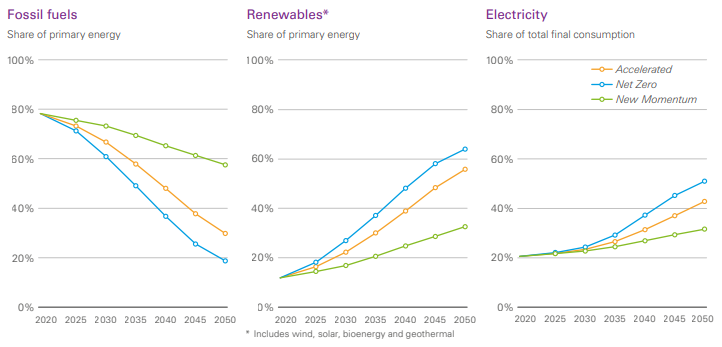
\includegraphics[width=160mm]{images/fig4.png}
    \fonte{\textit{British Petroleum Energy Outlook} \cite{bP2022}.}
\end{figure}
\end{comment}

%%petróleo Brasil - contexto atual 

O petróleo é a principal fonte de energia, fornecendo o combustível necessário para manter em funcionamento os diferentes meios de transporte \cite{gauto2016petroleo}. 
Após a pandemia de COVID, o valor do barril de petróleo se  manteve dentro da faixa de preços de US\$80 a US\$95, com início do conflito entre a Rússia e a Ucrânia o preço do barril de petróleo ultrapassou US\$140 \cite{ozili2022global}. 

De acordo com dados da Agência Nacional do Petróleo, Gás Natural e Biocombustíveis \cite{ANP2022}, a produção total de petróleo e gás natural no Brasil em abril de 2022 foi de 2,999 MMbbl/d (milhões de barris por dia) e 137 MMm3/d (milhões de metros cúbicos por dia), respectivamente. Essa produção foi proveniente de  6.089 poços, sendo 447 marítimos e 5.642 terrestres. A produção do pré-sal correspondeu a 75,4\% desse total e foi oriunda de 129 poços marítimos. Na Figura \ref{fig:Hu2018} apresenta um gráfico em colunas, o eixo das ordenadas presenta a quantidade em  MMbbl/d (milhões de barris por dia), o eixo da abcissas presenta o mês e ano da produção, os  dados mostram uma estabilidade na produção brasileira.

%%petróleo Brasil - descrição figura 2
\begin{figure}[H]
    \centering
    \caption{Histórico de produção de gás natural}. 
    \label{fig:Hu2018}
    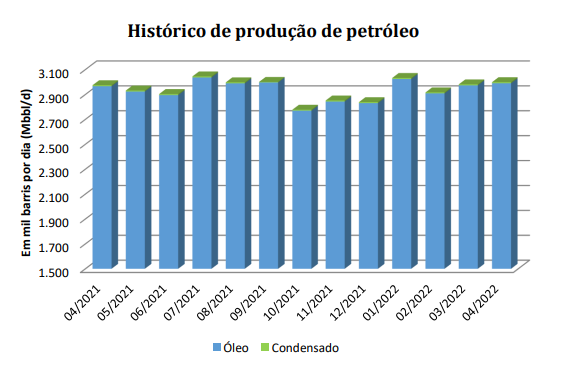
\includegraphics[width=130mm]{images/fig5.png}
    \fonte{Agência Nacional do Petróleo, Gás Natural e Biocombustíveis\cite{ANP2022}.}
\end{figure}

%%petróleo  - Anomalias  
Na industria do petróleo, é possível a ocorrência de eventos indesejados denominados anomalias. Por exemplo, o hidrato na linha de produção é uma anomalia, provocada pelo acúmulo de um composto cristalino formado por água e gás natural, que se assemelha a gelo  \cite{vargas2019base}, essa anomalia pode gerar perdas de produção durante dias ou até semanas, em alguns casos a desobstrução da linha é exigida, e a sonda marítima pode custar mais de 500 mil dólares ao dia \cite{andreolli2016introduccao}.  A detecção de anomalias é uma classificação do tipo binária (entre normalidade e anormalidade), na qual identifica-se a ocorrência de anomalia, porém sem especificá-la \cite{vargas2019base}.


%O monitoramento de processos industriais orientado a dados aplica estatísticas multivariadas e métodos de aprendizado de máquina para detectar e classificar anomalias em processos operacionais.
%% aprendizado de maquina
Na área de aprendizado de máquina, o problema de classificação pode ser definido como a categorização de uma determinada entrada em uma ou mais classes discretas e pré-definidas \cite{kadhim2019survey}. Em muitos processos industriais, busca-se detectar padrões raros, nos quais a maioria das observações referem-se a situações de normalidade, e a minoria, às situações raras que se deseja identificar \cite{santos2016literature}.



%% DESCRIÇÃO DO PROBLEMA 
\section{O PROBLEMA}

A indústria petrolífera possui um amplo monitoramento dos seus poços de petróleo, gerando assim uma grande quantidade de dados, esses dados estão disposto em MTS (do inglês \textit{Multivariate Time Series}, em português series temporais multivariadas) \cite{ismail2019deep}. Nas duas últimas décadas, a classificação de séries temporais tem sido considerada como um dos problemas mais desafiadores em mineração de dados.
O problema que motivou este trabalho é como detectar e classificar anomalias em poços petróleo por \textit{Multivariate Time Series}, em menor tempo de treinamento e com maior Acurácia do que os trabalhos correlatos identificados até o momento. 

Segundo \cite{rodrigo2021} o uso de técnica de redução de dimensão em problemas de detecção e classificação de anomalias em poços de produção de petróleo offshore apresentam resultados satisfatórios.

%% REDUÇÃO DE DIMENSIONALIDADE
No aprendizado de máquina, a alta dimensionalidade dos dados pode levantar problemas na precisão da classificação, reconhecimento de padrões e visualização. Treinamento em dados de alta dimensão podem se tornar difíceis devido à complexidade dos dados, o que pode levar ao que é chamado de maldição da dimensionalidade (do inglês,  \textit{Curse of Dimensionality}), como contramedida  muitas técnicas de redução de dimensionalidade foram propostas \cite{nanga2021review}.

\begin{comment}
\begin{figure}[H]
	\centering
	\caption{Plataforma de produção do pré-sal.}
	\label{fig:exemplo_sumarizacao_java}
	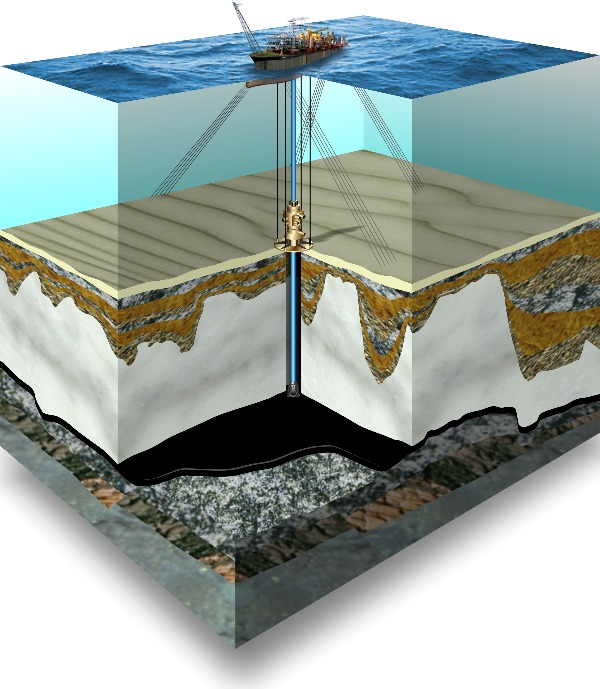
\includegraphics[width=105mm] 
	{images/plataforma.jpg}
	\fonte{Paulo Cabral/Banco de imagens da Petrobras.}
\end{figure}
\end{comment}

%% DESCRIÇÃO DA PROSPOSTA DO TRABALHO


\section{A PROPOSTA}
A hipótese deste trabalho é que aplicando técnicas de redução de dimensionalidade, podemos obter uma melhor acurácia do classificador do que a solução sem as técnicas de redução de dimensionalidade.

A proposta deste trabalho é utilizar três  técnicas de redução de dimensionalidade: KPCA (Análise de componentes principais do kernel, em inglês \textit {Kernel Principal Component Analysis}) \cite{nanga2021review}, ISOMAP (Mapeamento isométrico, em inglês \textit{Isometric Mapping}) \cite{jia2022iso}, e DMT (Transformação múltipla profunda , em inglês \textit{Deep Manifold Transformation}) \cite{li2020DTM}.

A base de dados a ser usada nos experimentos é a 3W \textit{dataset} \cite{vargas2019base}. Seguindo o trabalho de \citeonline{fernandes2022comparaccao} e \citeonline{junior2020detecccao}, serão usados os algoritmos de detecção de anomalias de classe única: Floresta de Isolamento (em inglês \textit{Isolation Forest}), Máquina de Vetor de Suporte de Classe Única (OCSVM do inglês, \textit{Oneclass Support Vector Machine}), Fator de Anomalia Local (LOF do inglês \textit{Local Outlier Factor}), Envelope Elíptico (MCD, do inglês \textit{Minimum Covariance Determinant}) e redes neurais do tipo \textit{Autoencoder} com camadas \textit{feedforward} e recorrentes do tipo LSTM (\textit{Long Short-Term Memory}). 

A métrica de comparação utilizada será  O F1-score é uma técnica simples que mede a discriminação de dois conjuntos de números reais\cite{F1akay2009support}, variando entre 0 e 1, Os resultados do uso de técnicas de redução de dimensionalidade serão comparados contra os resultados obtidos por  \citeonline{fernandes2022comparaccao} e \citeonline{junior2020detecccao}, que não usam esta etapa em sua solução.


%% DESCRIÇÃO DO PROBLEMA GERAL 
\section{OBJETIVO GERAL}
A ideia central da dissertação é a detecção de anomalias em poços de petróleo marítimos do tipo surgente, aplicando técnicas de redução de dimensionalidade.

%% DESCRIÇÃO DO OBJETIVOS 
\section{OBJETIVOS ESPECÍFICOS}
Para se alcançar o objetivo geral, os seguintes objetivos específicos serão realizados:
%% INICIO LISTA OBJETIVOS ESPECÍFICOS  
\begin{enumerate}

	\item {Realizar levantamento bibliográfico de trabalhos correlatos sobre Redução de dimensionalidade;}

	\item {Realizar levantamento bibliográfico sobre algoritmos de técnicas de redução de dimensionalidade }

	\item {Aplicar técnicas de redução de dimensionalidade:  KPCA (Análise de componentes principais do kernel, em inglês \textit {Kernel Principal Component Analysis}) \cite{nanga2021review}, ISOMAP (Mapeamento isométrico, em inglês \textit{Isometric Mapping}) \cite{jia2022iso}, e DMT (Transformação múltipla profunda , em inglês \textit{Deep Manifold Transformation}) \cite{li2020DTM}, ao 3W \textit{dataset}, para detecção de anomalias em poços de petróleo do tipo surgente;\cite{vargas2019base}}.
	
	\item {Aplicar técnicas detecção de anomalias de classe única:  Floresta de Isolamento (em inglês \textit{Isolation Forest}), Máquina de Vetor de Suporte de Classe Única (OCSVM do inglês, \textit{Oneclass Support Vector Machine}), Fator de Anomalia Local (LOF do inglês \textit{Local Outlier Factor}), Envelope Elíptico (MCD, do inglês \textit{Minimum Covariance Determinant}) e redes neurais do tipo \textit{Autoencoder} com camadas \textit{feedforward} e recorrentes do tipo LSTM (\textit{Long Short-Term Memory}} proposta por \cite{fernandes2022comparaccao}. 

    
    \item {Comparar os resultados obtidos após as utilização das técnicas de redução de dimensionalidade, com os resultados obtidos anteriormente por \cite{fernandes2022comparaccao}}, por meio da métrica F1-score .
    

\end{enumerate}
%% FIM  LISTA OBJETIVOS ESPECÍFICOS  


%% ORGANIZAÇÃO DO TRABALHO  
\section{ORGANIZAÇÃO DO TRABALHO}

Além deste capítulo introdutório, o restante deste documento está organizado em mais 3 capítulos. 
No Capítulo 2 será apresentado alguns trabalhos relacionados, sendo discutido as técnicas que foram utilizadas, os \textit{corpora} adotados e as medidas de avaliação para validar as propostas.
No Capítulo 3, será apresentada a proposta inicial deste trabalho, sendo discutido seus principais módulos e técnicas que serão exploradas.
Além disso, serão apresentados os corpora selecionados e as medidas de avaliação que serão adotadas para avaliar a abordagem proposta neste trabalho.
Por fim, no Capítulo 4, é apresentado o cronograma para execução do projeto de pesquisa.

% ---
% ------------------------ Referencial Teórico ------------------------
% ---

\chapter[REFERENCIAL TEÓRICO]{REFERENCIAL TEÓRICO} \label{cap:referencial}

\section{TRABALHOS CORRELATOS}

A base de dados publica 3w foi elaborada por \cite{vargas2019base}, será utilizada como base para aplicação dos algoritmos de redução dimensionalidade não lineares, conforme foi sugerido como trabalhos futuros por \cite{vargas2019base} na sua tese. O autor ainda elaborou um
\textit{benchmark} para detecção de anomalias usando as técnicas de Floresta de Isolamento e OCSVM.

No trabalho de \cite{fernandes2022comparaccao} foi  utilizado o \textit{benchmark} para detecção de anomalias proposto por \cite{vargas2019base}, estendeu seus resultados pois usou mais classificadores (LOF, Envelope Elíptico, Floresta de Isolamento, OCSVM e Redes Neurais do tipo \textit{autoencoders}), nesse trabalho não foi utilizada nenhuma técnica de redução de dimensionalidade, e ele será a base de comparação dos resultados obtidos com as técnicas de dimensionalidade propostas nesse trabalho.

No trabalho elaborado por \cite{rodrigo2021}, utilizou a base de dados pública 3w elaborada por \cite{vargas2019base} para detecção de anomalias, nesse trabalho é observado a etapa de redução de dimensionalidade utilizado a técnica de \textit{autoencoders}, onde os resultados obtidos foram de dezoito pontos percentuais para os modelos OCSVM e dez pontos percentuais para os modelos de Floresta de Isolamento \cite{rodrigo2021},  em comparação com o \textit{benchmark} proposto por\cite{vargas2019base}.



%%% INICIO PARTE REVISÃO
\todo[inline]{INICIO -  APENAS TEXTO BASE }

\section{REDUÇÃO DE DIMENSIONALIDADE}

Após a extração de características, é possível que se tenha uma grande quantidade de características, e pode ser necessário reduzir os custos de processamento. Esse processo é denominado de redução de dimensionalidade. Esta etapa não existiu na abordagem proposta
deste trabalho.
As técnicas mais comuns de redução de dimensionalidade são PCA (Principal Componet Analysis), LDA (Linear Discriminant Analysis) e NMF (Non-negative matrix factorization) (KOWSARI et al., 2019). O Self-Organizing Map (SOM) é um tipo específico de rede neural,
proposto por Kohonen (2013), que também é utilizado como uma ferramenta de redução de
dimensionalidade para extração de características em classificação de dados de alta
dimensionalidade, sendo considerado como uma alternativa ao PCA na detecção e diagnóstico
de falhas para processos industriais complexos (YU et al., 2014).

\subsection{TÉCNICAS DE REDUÇÃO DE DIMENSIONALIDADE NÃO LINEARES}

\subsubsection{KERNEL PRINCIPAL COMPONENT ANALYSIS (KPCA)}
é uma técnica de redução de dimensão não linear (NLDRT) que foi introduzida por. É uma extensão do PCA tradicional que funciona com espaço de recursos de alta dimensão (HD) empregando o método kernel. A diferença entre KPCA e PCA é que existe um cálculo de vetor próprio da matriz kernel com KPCA enquanto o PCA calcula a matriz de covariância [195]. Além disso, componentes principais não lineares podem ser extraídos com menos poder computacional com KPCA. Para dados com variedades não lineares, KPCA oferece boa codificação [196]. Com KPCA, há uma transformação não linear dos dados de entrada do espaço de entrada original para o kernel para cada dado. Uma matriz kernel K é então formada a partir do produto interno do novo recurso. A PCA é consequentemente aplicado o K centralizado na estimação da matriz de covariância dos novos vetores de características [197]. Alguns kernels extensivamente usados incluem Gaussiano, Polinomial e Tangente Hiperbólico e Radial. Uma desvantagem do KPCA é que o custo de computação pode ser extremamente alto, o que pode levar a problemas numéricos de diagonalização de grandes matrizes [197]. Para superar essas desvantagens, Rosipal e Girolami propuseram um algoritmo EM para KPCA [197], que é uma abordagem de maximização de expectativas para realizar análise de componentes principais do kernel e resultados experimentais mostraram que é um método computacionalmente eficiente, especialmente para um grande número de pontos de dados. Uma desvantagem dessa abordagem, no entanto, é que ela ainda precisa armazenar a matriz do kernel N × N, o que limita sua aplicabilidade em muitos problemas de grandes conjuntos de dados. O Block Adaptive KPCA (BAKPCA) foi desenvolvido por  para adicionar novos blocos de forma não iterativa e dinâmica e remover blocos de dados antigos. É eficiente no processamento de sinais e também no monitoramento de processos. O Greedy KPCA também foi proposto por [199] para melhorar o desempenho do classificador SVM. Os resultados mostraram que o kernel ganancioso PCA pode reduzir significativamente a complexidade enquanto mantém a precisão da classificação. No entanto, o Greedy KPCA foi considerado inadequado para remoção de ruído. O Subconjunto KPCA (SKPCA) também foi introduzido por [200] para reduzir complexidades nos cálculos de KPCA para redução de dimensão, bem como classificação. O Robust KPCA também foi proposto por [201] para lidar com outliers e melhorar a precisão da classificação de proteínas. [202] introduziram o PCA discriminativo (dPCA) para análise discriminativa de múltiplos S. Nanga et al. DOI: 10.4236/jdaip.2021.93013 201 Journal of Data Analysis and Information Processing datasets e tem sido aplicado em áreas como dados de saúde, dados de sensores e imagens faciais. A construção supervisionada do kernel para PCA não supervisionado no reconhecimento facial também foi proposta. Os resultados experimentais revelaram que a construção do kernel supervisionado para PCA não supervisionado (SK-PCA) teve um desempenho melhor do que o KPCA com kernel RBF (RBF-PCA) usando bancos de dados ORL e FERET. Os tipos de dados citados na literatura nos quais o KPCA foi aplicado e teve um bom desempenho são Imagem, Áudio , Vídeo e dados de séries temporais.

\subsubsection{ISOMETRIC MAPPING (ISOMAP)}

Outro NLDRT não supervisionado popular cujo objetivo é encontrar intrinsecamente estruturas de dados de uma variedade não linear é o ISOMAP. O algoritmo proposto por [227] tenta extrair parametrizações para conjuntos de dados em um espaço de baixa dimensão para formar um espaço de alta dimensão tal que haja uma preservação das distâncias geodésicas pareadas de modo que pontos próximos estejam distantes no mapa de espaço de alta dimensão para pontos próximos que estão distantes no espaço de baixa dimensão. A característica distintiva do ISOMAP é sua capacidade de obter uma representação dimensional menor dos dados, enquanto a distância geodésica é preservada [227]; [228]. O ISOMAP combina as principais características do PCA e do MDS em termos de eficiência computacional, garantias de convergência assintótica e otimização global com a flexibilidade de uma extensa classe de manifolds não lineares. A abordagem ISOMAP baseia-se basicamente no MDS tradicional, mas a propriedade distintiva é que procura preservar a geometria intrínseca dos dados que são capturados na distância geodésica entre os pares de pontos de dados [227]. O ISOMAP tem sido eficiente quando usado na detecção de irregularidades de análises de vídeo em tempo real [229]. Um ISOMAP baseado em caminho foi proposto por [230] para melhorar a memória e também as complexidades de tempo. O caminho geodésico é usado nesta abordagem para encontrar a incorporação de baixa dimensão. Algumas das desvantagens do ISOMAP são que ele é computacionalmente caro e tem um desempenho ruim quando o manifold não é bem amostrado e contém furos [230]. O Landmark Isomap (L-Isomap) foi apresentado por [231] para melhorar a escalabilidade do Isomap. O ISOMAP foi aplicado com sucesso na condição do tráfego rodoviário urbano [232], sumarização de fala e identificação de rachaduras em materiais [233], reconhecimento facial [234]. Versões supervisionadas do Isomap foram propostas. Isso inclui Isomap Supervisionado para classificação, Isomap Supervisionado com medidas de dissimilaridade na aprendizagem incorporada e Isomap Supervisionado para classificação de imagem de folha de planta [237].

Fig. \ref{fig:ISOMAP} Diagrama esquemático do algoritmo ISOMAP.
  Nota: A: Distância Euclidiana e Distância Geodésica;
  B: diagramas de pontos adjacentes;
C: reduzido a dados bidimensionais.
Uma distância euclidiana (comprimento da linha tracejada) do espaço de entrada de alta dimensão e distância geodésica da variedade de baixa dimensão (comprimento da curva sólida);
B o verdadeiro caminho geodésico no mapa geodésico que é efetivamente calculado através do gráfico de vizinhança G e este caminho é tomado como o caminho mais curto.
  C a incorporação bidimensional recuperada pelo ISOMAP, onde as linhas azuis na

\begin{figure}[H]
    \centering
    \caption{Diagrama esquemático do algoritmo ISOMAP.}. 
    \label{fig:ISOMAP}
 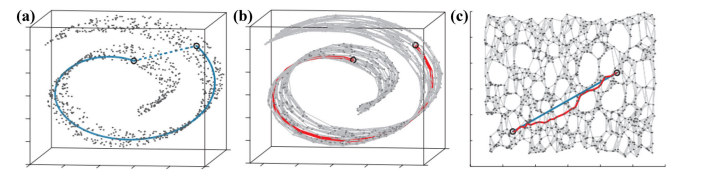
\includegraphics[width=120mm]{images/fig8.png}
    \fonte{\cite{jia2022iso}}
\end{figure}


\subsubsection{DEEP MANIFOLD TRANSFORMATION(DMT)}

é uma rede neural profunda de feed-forward regularizada por restrições de camada cruzada. Uma instância da arquitetura DMT é ilustrada na Fig.1 usando um DMT-AutoEncoder. De um modo geral, uma rede não linear de várias camadas pode suportar um grau mais alto de não linearidade do que redes não lineares de camada única ou equivalentes como t-SNE ou UMAP. O NLDR é realizado usando o DMT-Encoder, que transforma a entrada X em uma incorporação (no espaço latente) Z = X(L) na camada L (a camada latente). Os recursos latentes Z podem ser usados para tarefas posteriores, como visualização e classificação. O DMT-Decoder, que pode assumir uma forma simétrica ao DMT-Encoder, é treinado com as restrições de reconstrução (linhas tracejadas laranja) para reconstruir Z em Xˆ. O codificador DMT aprendido pode ser aplicado.

Figura \ref{fig:li2020DTM}: Ilustração da estrutura de transformação profunda do manifold (DMT) usando um DMT-AutoEncoder (melhor visualizado em cores). Consiste em uma cascata de transformações  (l) (ou ˆ(l) , setas azuis) com as restrições de preservação de geometria local (LGP) entre camadas (mostradas em arcos laranja) impostas entre a camada 0 e a camada L com peso . A restrição de perda de reconstrução com peso  é mostrada em linha tracejada laranja.

\begin{figure}[H]
    \centering
    \caption{Deep manifold transformation (DMT).}. 
    \label{fig:li2020DTM}
 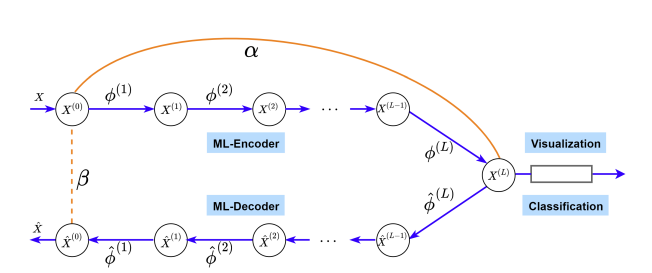
\includegraphics[width=150mm]{images/fig7.png}
    \fonte{\cite{li2020DTM}}
\end{figure}







% ---
% ------------------------ Desenvolvimento ------------------------
% ---
\chapter[MATERIAIS E MÉTODOS]{MATERIAIS E MÉTODOS}

Neste capítulo apresentam-se os métodos empregados na proposta deste trabalho. Um processo de classificação, conforme ilustrado na Figura \ref{fig:4}, pode ser dividido em seis etapas \cite{kadhim2019survey}: coleta de dados, pré-processamento, extração de características, redução de dimensionalidade, aplicação da técnica de classificação e avaliação de desempenho.

\begin{figure}[H]
    \centering
    \caption{Etapas do processo de classificação}. 
    \label{fig:4}
 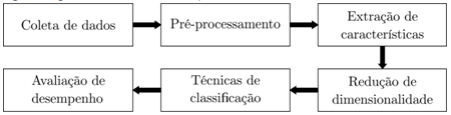
\includegraphics[width=120mm]{images/fig6.png}
    \fonte{Adaptado de \cite{kadhim2019survey}.}
\end{figure}

%% INICIO DESCRIÇÃO BASE DE DADOS
\section{BASES DE DADOS}
A base de dados utilizada 3W dataset (VARGAS et al., 2019) é pública e contém 1.984
instâncias de séries temporais da produção de poços de petróleo marítimos do tipo surgente
(poços que conseguem escoar os fluidos produzidos até a plataforma com sua própria
pressão). Essas instâncias foram separadas em: operação em condições normais e anomalias.
As anomalias foram organizadas em oito classes. Essa base pode ser utilizada tanto para
detecção quanto para classificação de anomalias em poços de petróleo.


%% INICIO PRÉ-PROCESSAMENTO
\section{PRÉ-PROCESSAMENTO}
A etapa de pré-processamento trata da preparação inicial do conjunto de dados coletado. No
caso de séries temporais, nessa etapa, inclui-se a análise dos dados, geração de gráficos para
entendimento do dados, remoção de valores nulos e/ou congelados e re-amostragens de
observações das séries temporais para balanceamento da base de dados.

%% INICIO PRÉ-PROCESSAMENTO
\section{EXTRAÇÃO DE CARACTERÍSTICAS }
A partir de cada amostra de série temporal, foram extraídas e utilizadas como características a
mediana, média, desvio padrão, variância, máximo e mínimo para cada variável. Para esta
extração de características das séries temporais foi utilizada a biblioteca tsfresh2
(Time seriesfeature extraction) (CHRIST et al., 2018) na configuração de parâmetros mínimos, de forma a
ser possível reproduzir os resultados iniciais gerados por Vargas (2019).

\begin{figure}[H]
    \centering
    \caption{Descrição das variáveis das séries temporais presentes no 3W dataset}. 
    \label{fig:10}
 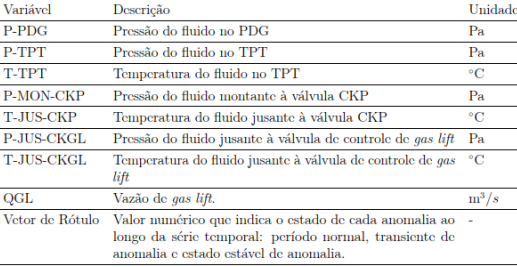
\includegraphics[width=120mm]{images/fig10.png}
    \fonte{\cite{vargas2019base}}
\end{figure}


%% INICIO REDUÇÃO DE DIMENSIONALIDADE
\section{REDUÇÃO DE DIMENSIONALIDADE}
Após a extração de características, é possível que se tenha uma grande quantidade de
características, e pode ser necessário reduzir os custos de processamento. Esse processo é
denominado de redução de dimensionalidade.Foram utilizadas as seguintes tecnicas:

\subsection{KERNEL PRINCIPAL COMPONENT ANALYSIS (KPCA)}
\subsection{ISOMETRIC MAPPING (ISOMAP)}
\subsection{DEEP MANIFOLD TRANSFORMATION(DMT)}


%% INICIO TÉCNICAS DE CLASSIFICAÇÃO
\section{TÉCNICAS DE CLASSIFICAÇÃO}

%% INICIO AVALIAÇÃO DE DESEMPENHO
\section{AVALIAÇÃO DE DESEMPENHO}
Na última etapa do processo de classificação, é necessário avaliar o desempenho obtido. De
acordo com Kowsari et al. (2019), essa avaliação é geralmente feita por meio de métricas, tais
como acurácia, revogação, precisão ou por meio do indicador medida-F1. Estas métricas são
obtidas a partir da matriz de confusão, ilustrada na Tabela 4, na qual são listados os valores
verdadeiros positivos (ou True Positive - TP), falsos positivos (ou False Positive FP),
verdadeiros negativos (ou True Negative - TN) e falsos negativos (ou False Negative - FN)
para cada classe.
Nesse trabalho, foi utilizada a métrica de medida F1 para análise de desempenho. Os testes
estatísticos de Friedman e Wilcoxon também foram aplicados aos resultados dos
experimentos de forma a permitir comparações entre os classificadores entre si e com os
resultados do trabalho de Vargas (2019).
%%% INICIO PARTE REVISÃO
\todo[inline]{FIM -  APENAS TEXTO BASE }

\chapter[CRONOGRAMA]{CRONOGRAMA}

\begin{table}[!ht]
    \label{fig:cronograma_1}
    \centering
    \caption{Cronograma}
    \centering    
    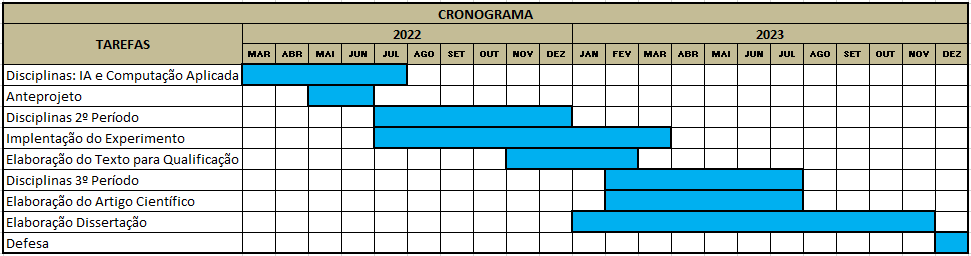
\includegraphics[width=160mm]{images/cronograma.png}
    \fonte{Elaborado pelo Autor (2022).}
\end{table}



%\include{tex/Cap5-materiaisemetodos}

% ---
% ------------------------ Resultados ------------------------
% ---
%\include{tex/Cap4-resultados}

% ----------------------------------------------------------
% Finaliza a parte no bookmark do PDF
% para que se inicie o bookmark na raiz
% e adiciona espaço de parte no Sumário
% ----------------------------------------------------------
\phantompart

% ---
% ------------------------ Conclusão ------------------------
% ---
%\include{tex/Cap6-conclusao}
% ---



% ----------------------------------------------------------
% ELEMENTOS PÓS-TEXTUAIS
% ----------------------------------------------------------
\postextual
% ----------------------------------------------------------

% ----------------------------------------------------------
% Referências bibliográficas
% ----------------------------------------------------------
\renewcommand{\bibname}{REFERÊNCIAS}
\citeoption{abnt-full-initials=yes}

\bibliography{references}

% ----------------------------------------------------------
% Glossário
% ----------------------------------------------------------
%
% Consulte o manual da classe abntex2 para orientações sobre o glossário.
%
%\glossary


% ----------------------------------------------------------
% Apêndices
% ----------------------------------------------------------

% ---
% Inicia os apêndices
% ---


%%% Início dos apêndices ---------------------------------------------
\apendices
%%% A linha abaixo impede que as seções, subseções, etc. dos apêndices e anexos
%%% sejam mostradas no Sumário.
\addtocontents{toc}{\protect\setcounter{tocdepth}{0}}

%\renewcommand{\apendicesname}{APÊNDICES}
%\partapendices*

% --------------------------------------------------------------------
%\settocpreprocessor{chapter}{}
%\chapter{Artigos por autor}

%\todo[inline]{Ricardo, termine de colocar a lista dos artigos. Complete os que estão faltando no bib}

Lista de artigos dos 20 autores mais produtivos na área de biometria por movimentos oculares: 

\begin{enumerate}[label=\arabic*.,ref=\arabic*]
    \item Komogortsev, O. V.:  
    \begin{enumerate}[label*=\arabic*.,ref=\theenumi.\arabic*]
        \item \cite{holland2011biometric} \item \cite{komogortsev2012biometric} \item \cite{komogortsev2010biometric} \item \cite{holland2013complex} 
        \item \cite{kasprowski2012first} \item \cite{komogortsev2012multimodal} 
        \item \cite{holland2012biometric} \item \cite{holland2013complexb} \item \cite{komogortsev2015attack} \item \cite{komogortsev2013liveness} \item \cite{rigas2014biometric} 
        \item \cite{komogortsev2013biometric} \item \cite{komogortsev2014template} \item \cite{komogortsev2015bioeye} \item \cite{komogortsev2015biometrics} 
        \item \cite{komogortsev20132d} 
        \item \cite{komogortsev2012cue} 
        \item \cite{komogortsev2014application} 
        \item \cite{rigas2017current} 
        \item \cite{rigas2016towards} 
        \item \cite{rigas2016biometric} 
        \item \cite{rigas2015eye} 
        \item \cite{rigas2014biometric} 
        \item \cite{rigas2014gaze} 
        \item \cite{brooks2013perceptions} \item \cite{holland2014software} \item \cite{komogortsev2016oculomotor} 
        \item \cite{zemblys2018using} 
        \item \cite{abdulin2015person} 
        \item \cite{friedman2017method} 
        \item \cite{abdulin2016eye} 
        \item \cite{rigas2018study} 
        \item \cite{lohr2018implementation}        
    \end{enumerate}
    \item Rigas, I.:  
    \begin{enumerate}[label*=\arabic*.,ref=\theenumi.\arabic*]
        \item \cite{rigas2012biometric} 
        \item \cite{rigas2012human} 
        \item \cite{rigas2014biometric} 
        \item \cite{kasprowski2013influence} 
        \item \cite{komogortsev2015bioeye} 
        \item \cite{rigas2017current} 
        \item \cite{rigas2016towards} 
        \item \cite{rigas2016biometric} 
        \item \cite{rigas2015eye} 
        \item \cite{rigas2014biometric}
        \item \cite{rigas2014gaze}
        \item \cite{kasprowski212influence} 
        \item \cite{abdulin2016eye} 
        \item \cite{rigas2018study}	
    \end{enumerate}
    \item Kasprowski, P.: 
    \begin{enumerate}[label*=\arabic*.,ref=\theenumi.\arabic*]
        \item \cite{kasprowski2004eye} 
        \item \cite{kasprowski2012first} 
        \item \cite{kasprowski2014second} 
        \item \cite{kasprowski2005enhancing} 
        \item \cite{kasprowski2013impact} 
        \item \cite{kapczynski2006modern} 
        \item \cite{kasprowski2013influence} 
        \item \cite{kasprowski2004flick} 
        \item \cite{kasprowski2018fusion} 
        \item \cite{kasprowski2016using}
        \item \cite{harezlak2017eye} 
        \item \cite{kasprowski2016disk} 
        \item \cite{kasprowski212influence}			 
    \end{enumerate}
    \item Holland, C. D.: 
    \begin{enumerate}[label*=\arabic*.,ref=\theenumi.\arabic*]
        \item \cite{holland2011biometric} 
        \item \cite{holland2013complex} 
        \item \cite{komogortsev2012multimodal} 
        \item \cite{holland2012biometric} 
        \item \cite{holland2013complex} 
        \item \cite{komogortsev2015attack} 
        \item \cite{komogortsev2013biometric} 
        \item \cite{komogortsev2014template}
        \item \cite{komogortsev2015biometrics} 
        \item \cite{komogortsev20132d} 
        \item \cite{komogortsev2012cue} 
        \item \cite{komogortsev2014application}
        \item \cite{holland2014software} 
        \item \cite{komogortsev2016oculomotor}			 
    \end{enumerate}
    \item Karpov, A.: 
    \begin{enumerate}[label*=\arabic*.,ref=\theenumi.\arabic*]
        \item \cite{komogortsev2012biometric} 
        \item \cite{kasprowski2012first} 
        \item \cite{komogortsev2012multimodal} 
        \item \cite{komogortsev2015attack} 
        \item \cite{komogortsev2013liveness} 
        \item \cite{komogortsev2014template} 
        \item \cite{komogortsev2015biometrics} 
        \item \cite{komogortsev20132d} 
        \item \cite{komogortsev2012cue} 
        \item \cite{komogortsev2016oculomotor}			
    \end{enumerate}
    \item Juhola, M.:  
    \begin{enumerate}[label*=\arabic*.,ref=\theenumi.\arabic*]
        \item \cite{juhola2013biometric} 
        \item \cite{zhang2012biometric} 
        \item \cite{zhang2014biometricb} 
        \item \cite{zhang2015biometric} 
        \item \cite{zhang2017biometrics} 
        \item \cite{zhang2014biometric} 
        \item \cite{zhang2013applying}
    \end{enumerate}
    \item Zhang, Y.:  
    \begin{enumerate}[label*=\arabic*.,ref=\theenumi.\arabic*]
        \item \cite{juhola2013biometric} 
        \item \cite{zhang2012biometric} 
        \item \cite{zhang2014biometricb} 
        \item \cite{zhang2015biometric} 
        \item \cite{zhang2017biometrics} 
        \item \cite{zhang2014biometric} 
        \item \cite{zhang2013applying}			 
    \end{enumerate}
    \item Harezlak, K.:  
    \begin{enumerate}[label*=\arabic*.,ref=\theenumi.\arabic*]
        \item \cite{kasprowski2014second} 
        \item \cite{kasprowski2018fusion} 
        \item \cite{kasprowski2016using} 
        \item \cite{harezlak2017eye} 
        \item \cite{kasprowski2016disk}				 
    \end{enumerate}
    \item Deravi, F.:  
    \begin{enumerate}[label*=\arabic*.,ref=\theenumi.\arabic*]
        \item \cite{deravi2011gaze} 
        \item \cite{ali2013spoofing} 
        \item \cite{ali2018gaze} 
        \item \cite{ali213spoofing}			 
    \end{enumerate}
    \item Ali, A.: 
    \begin{enumerate}[label*=\arabic*.,ref=\theenumi.\arabic*]
        \item \cite{ali2013spoofing} 
        \item \cite{ali2018gaze} 
        \item \cite{ali213spoofing}
    \end{enumerate}
    \item Hansen, D. W.:  
    \begin{enumerate}[label*=\arabic*.,ref=\theenumi.\arabic*]
        \item \cite{hansen2010eye} 
        \item \cite{vitonis2014person} 
        \item \cite{batista2015depth}	
    \end{enumerate}
    \item Hoque, S.:  
    \begin{enumerate}[label*=\arabic*.,ref=\theenumi.\arabic*]
        \item \cite{ali2013spoofing} 
        \item \cite{ali2018gaze} 
        \item \cite{ali213spoofing}	
    \end{enumerate}
    \item Ober, J.:              
    \begin{enumerate}[label*=\arabic*.,ref=\theenumi.\arabic*]
        \item \cite{kasprowski2004eye} 
        \item \cite{kasprowski2005enhancing} 
        \item \cite{kasprowski2004flick}			 
    \end{enumerate}
    \item Saeed, U.:              
    \begin{enumerate}[label*=\arabic*.,ref=\theenumi.\arabic*]
        \item \cite{saeed2014survey} 
        \item \cite{saeed2016eye} 
        \item \cite{saeed2014automatic}			 
    \end{enumerate}
    \item Aragon, C. R.:           
    \begin{enumerate}[label*=\arabic*.,ref=\theenumi.\arabic*]
        \item \cite{komogortsev2012biometric} 
        \item \cite{komogortsev2010biometric} 
        \item \cite{brooks2013perceptions}			 
    \end{enumerate}
    \item Abdulin, E.:            
    \begin{enumerate}[label*=\arabic*.,ref=\theenumi.\arabic*]
        \item \cite{rigas2016towards} 
        \item \cite{abdulin2015person} 
        \item \cite{abdulin2016eye}			
    \end{enumerate}
    \item Awad, A.:               
    \begin{enumerate}[label*=\arabic*.,ref=\theenumi.\arabic*]
        \item \cite{rose2017biometric} 
        \item \cite{rose2017biometricb}			 
    \end{enumerate}
    \item Bednarik, R.:
    \begin{enumerate}[label*=\arabic*.,ref=\theenumi.\arabic*]
        \item \cite{bednarik2005eye} 
        \item \cite{kinnunen2010towards}				 
    \end{enumerate}
    \item Economou, G.:          
    \begin{enumerate}[label*=\arabic*.,ref=\theenumi.\arabic*]
        \item \cite{rigas2012biometric} 
        \item \cite{rigas2012human}			
    \end{enumerate}
    \item Fotopoulos, S.:        
    \begin{enumerate}[label*=\arabic*.,ref=\theenumi.\arabic*]
        \item \cite{rigas2012biometric} 
        \item \cite{rigas2012human}	
    \end{enumerate}
\end{enumerate}

\begin{comment}

\chapter{Matrizes de Confusão da Segunda Arquitetura}

% Please add the following required packages to your document preamble:
% \usepackage{graphicx}
\begin{table}[h]
\caption{Matriz de confusão da ResNET.}
\resizebox{\textwidth}{!}{%
\begin{tabular}{|l|l|l|l|l|l|l|l|l|l|l|l|l|l|l|l|l|l|l|l|l|l|l|l|l|l|l|l|l|l|}
\hline
   & 1 & 2  & 3 & 4  & 5 & 6 & 7 & 8 & 9 & 10 & 11 & 12 & 13 & 14 & 15 & 16 & 17 & 18 & 19 & 20 & 21 & 22 & 23 & 24 & 25 & 26 & 27 & 28 & 29 \\ \hline
1  & 3 & 1  & 0 & 0  & 0 & 0 & 0 & 0 & 0 & 0  & 0  & 0  & 0  & 0  & 0  & 1  & 0  & 0  & 0  & 0  & 1  & 0  & 1  & 0  & 1  & 0  & 3  & 0  & 1  \\ \hline
2  & 0 & 11 & 0 & 1  & 0 & 0 & 0 & 0 & 0 & 0  & 0  & 0  & 0  & 0  & 0  & 0  & 0  & 0  & 0  & 0  & 1  & 0  & 0  & 0  & 0  & 1  & 0  & 0  & 0  \\ \hline
3  & 0 & 0  & 5 & 0  & 2 & 0 & 0 & 0 & 0 & 0  & 1  & 0  & 0  & 0  & 0  & 0  & 0  & 0  & 0  & 0  & 0  & 0  & 0  & 0  & 0  & 1  & 0  & 0  & 0  \\ \hline
4  & 0 & 1  & 0 & 11 & 0 & 0 & 0 & 0 & 0 & 1  & 0  & 0  & 1  & 0  & 0  & 0  & 0  & 0  & 0  & 0  & 0  & 0  & 0  & 0  & 0  & 1  & 0  & 0  & 0  \\ \hline
5  & 0 & 0  & 0 & 0  & 1 & 0 & 0 & 0 & 1 & 0  & 1  & 1  & 0  & 0  & 0  & 1  & 0  & 0  & 0  & 1  & 1  & 0  & 0  & 0  & 0  & 0  & 0  & 0  & 0  \\ \hline
6  & 0 & 0  & 0 & 0  & 0 & 6 & 0 & 0 & 0 & 0  & 0  & 0  & 0  & 0  & 0  & 0  & 0  & 0  & 0  & 0  & 0  & 0  & 0  & 0  & 0  & 0  & 0  & 0  & 0  \\ \hline
7  & 0 & 1  & 0 & 1  & 0 & 0 & 2 & 0 & 0 & 0  & 1  & 0  & 0  & 1  & 0  & 1  & 0  & 1  & 2  & 2  & 0  & 1  & 0  & 0  & 0  & 1  & 0  & 0  & 0  \\ \hline
8  & 0 & 0  & 0 & 0  & 0 & 0 & 0 & 2 & 0 & 0  & 0  & 1  & 0  & 0  & 0  & 0  & 0  & 0  & 0  & 1  & 0  & 0  & 0  & 2  & 0  & 0  & 0  & 0  & 1  \\ \hline
9  & 1 & 0  & 0 & 0  & 0 & 0 & 0 & 0 & 1 & 1  & 0  & 0  & 0  & 0  & 0  & 0  & 0  & 1  & 0  & 2  & 0  & 0  & 0  & 2  & 0  & 0  & 0  & 0  & 0  \\ \hline
10 & 0 & 0  & 0 & 0  & 0 & 0 & 0 & 1 & 0 & 3  & 0  & 0  & 0  & 0  & 1  & 3  & 0  & 0  & 2  & 0  & 0  & 0  & 0  & 1  & 1  & 0  & 0  & 0  & 0  \\ \hline
11 & 0 & 1  & 1 & 0  & 2 & 0 & 0 & 0 & 0 & 0  & 1  & 0  & 0  & 0  & 0  & 0  & 0  & 0  & 0  & 0  & 0  & 0  & 0  & 1  & 0  & 0  & 0  & 0  & 0  \\ \hline
12 & 0 & 0  & 0 & 0  & 1 & 0 & 0 & 0 & 1 & 0  & 0  & 2  & 1  & 0  & 1  & 1  & 0  & 1  & 0  & 3  & 0  & 0  & 1  & 0  & 0  & 1  & 0  & 3  & 0  \\ \hline
13 & 0 & 0  & 0 & 0  & 0 & 0 & 0 & 0 & 0 & 1  & 0  & 0  & 5  & 0  & 2  & 0  & 0  & 0  & 0  & 0  & 0  & 0  & 1  & 0  & 0  & 0  & 0  & 0  & 0  \\ \hline
14 & 0 & 2  & 0 & 5  & 0 & 0 & 0 & 0 & 0 & 0  & 0  & 0  & 0  & 1  & 1  & 0  & 0  & 0  & 0  & 0  & 0  & 0  & 0  & 0  & 0  & 1  & 0  & 0  & 0  \\ \hline
15 & 0 & 0  & 0 & 0  & 0 & 0 & 1 & 0 & 0 & 1  & 0  & 0  & 0  & 1  & 4  & 0  & 0  & 1  & 0  & 0  & 0  & 0  & 0  & 0  & 0  & 0  & 0  & 0  & 0  \\ \hline
16 & 0 & 0  & 0 & 0  & 1 & 0 & 0 & 0 & 0 & 0  & 0  & 0  & 0  & 0  & 0  & 2  & 0  & 1  & 0  & 2  & 0  & 0  & 0  & 0  & 0  & 0  & 0  & 0  & 0  \\ \hline
17 & 2 & 1  & 0 & 2  & 0 & 0 & 0 & 0 & 0 & 0  & 0  & 0  & 0  & 0  & 0  & 2  & 2  & 0  & 0  & 0  & 1  & 0  & 1  & 0  & 0  & 0  & 0  & 0  & 0  \\ \hline
18 & 0 & 0  & 0 & 0  & 0 & 4 & 0 & 0 & 0 & 0  & 1  & 0  & 0  & 0  & 0  & 0  & 0  & 2  & 0  & 0  & 0  & 0  & 2  & 0  & 0  & 0  & 0  & 0  & 0  \\ \hline
19 & 0 & 1  & 0 & 0  & 0 & 0 & 0 & 1 & 0 & 0  & 0  & 1  & 0  & 1  & 0  & 0  & 0  & 0  & 2  & 0  & 0  & 0  & 0  & 1  & 0  & 0  & 0  & 0  & 2  \\ \hline
20 & 0 & 0  & 0 & 0  & 0 & 0 & 0 & 0 & 2 & 0  & 0  & 0  & 0  & 0  & 0  & 0  & 0  & 0  & 0  & 6  & 0  & 0  & 0  & 1  & 0  & 0  & 0  & 0  & 0  \\ \hline
21 & 0 & 0  & 0 & 0  & 0 & 0 & 0 & 0 & 0 & 0  & 0  & 0  & 0  & 0  & 0  & 0  & 0  & 1  & 0  & 0  & 4  & 0  & 0  & 0  & 0  & 0  & 0  & 0  & 0  \\ \hline
22 & 0 & 2  & 0 & 2  & 0 & 0 & 0 & 0 & 0 & 0  & 0  & 0  & 1  & 1  & 0  & 0  & 0  & 0  & 0  & 0  & 0  & 2  & 0  & 0  & 0  & 1  & 0  & 0  & 0  \\ \hline
23 & 1 & 0  & 0 & 0  & 0 & 1 & 0 & 0 & 0 & 0  & 0  & 0  & 1  & 0  & 0  & 0  & 0  & 1  & 0  & 1  & 0  & 0  & 2  & 0  & 1  & 0  & 1  & 0  & 0  \\ \hline
24 & 0 & 0  & 0 & 0  & 0 & 1 & 0 & 2 & 0 & 0  & 0  & 0  & 0  & 0  & 0  & 0  & 0  & 0  & 0  & 0  & 0  & 0  & 0  & 8  & 0  & 0  & 0  & 0  & 0  \\ \hline
25 & 0 & 0  & 0 & 2  & 0 & 0 & 0 & 0 & 0 & 1  & 0  & 0  & 0  & 0  & 0  & 0  & 0  & 0  & 0  & 1  & 0  & 0  & 1  & 0  & 6  & 0  & 0  & 1  & 1  \\ \hline
26 & 0 & 1  & 0 & 0  & 0 & 0 & 0 & 0 & 0 & 0  & 0  & 0  & 1  & 0  & 0  & 0  & 0  & 0  & 0  & 0  & 0  & 0  & 0  & 0  & 0  & 9  & 0  & 0  & 0  \\ \hline
27 & 2 & 3  & 0 & 0  & 0 & 0 & 0 & 0 & 0 & 0  & 0  & 0  & 1  & 0  & 0  & 0  & 0  & 0  & 0  & 0  & 0  & 0  & 3  & 0  & 0  & 1  & 5  & 0  & 1  \\ \hline
28 & 1 & 0  & 0 & 0  & 0 & 0 & 0 & 0 & 1 & 0  & 0  & 0  & 0  & 0  & 0  & 1  & 0  & 1  & 1  & 0  & 0  & 0  & 1  & 0  & 2  & 0  & 0  & 5  & 0  \\ \hline
29 & 0 & 1  & 0 & 0  & 0 & 0 & 0 & 0 & 0 & 0  & 1  & 0  & 0  & 0  & 0  & 1  & 1  & 0  & 1  & 0  & 0  & 0  & 0  & 0  & 0  & 0  & 1  & 0  & 3  \\ \hline
\end{tabular}%
}
\label{tab:matriz_resnet}
\fonte{Elaborado pelo autor (2019).}
\end{table}

\end{comment}





%---------------------------------------------------------------------
% INDICE REMISSIVO
%---------------------------------------------------------------------
\phantompart

%---------------------------------------------------------------------

\end{document}